%----------------------------------------------------------------
% Form coordinates.tex

\begin{figure}[!b]
  \centering
  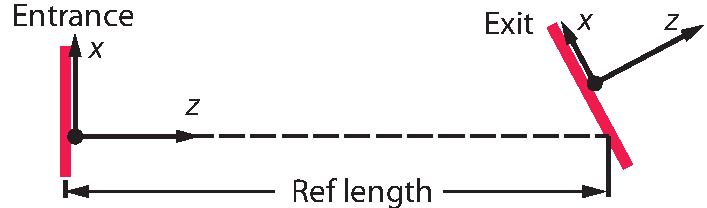
\includegraphics[width=5in]{patch-coords.pdf}
  \caption[The coordinate system for a patch element.]
{The coordinate system for a patch element. The thick red lines
delineate the entrance and exit planes. Within the \vn{patch}, the reference
orbit is a straight line coinciding with the $z$ axis of the entrance coordinate.}
  \label{f:patch.coords}
\end{figure}

\index{patch!coordinate system}
\index{floor_shift!coordinate system}
\index{wiggler!coordinate system}
\index{reference length}\index{s-length}
The reference orbit for a \vn{patch} element is shown in
\fig{f:patch.coords}.  Within the \vn{patch}, the reference orbit is
a straight line coinciding with the $z$ axis of the entrance
coordinate. The \vn{patch} has associated with it two longitudinal
lengths: 
\begin{itemize}
\item
The ``reference length'' is the length that the reference particle
travels from the entrance plane to the exit plane. The reference
length is used to determine the change in the reference time through
the \vn{patch} which, in turn, is used to calculate the change in the
phase space $z$ coordinate (cf.~\Eq{zbctt}). With the reference length
so chosen, the change in $z$ of a particle entering the \vn{patch} on
the zero-orbit will be zero.
\item
The ``S-length'' is the length of the patch when the $s$-positions of
the elements are calculated. The S-length is the longitudinal distance
from the entrance origin to the exit origin. The S-length is the same
at the \vn{z_offset} attribute of the \vn{patch} and is also the same
as the \vn{l} length attribute (\sref{s:l}). The S-length is used when
calculating the track of a particle through a patch. That is, when
\bmad calculates the trajectory of a particle transversing a patch,
the dependent $s$ position (relative to the beginning of the
\vn{patch}) will vary from 0 to S-length. At $s = 0$ the particle is
at the entrance face of the \vn{patch}. Between $s = 0$ and $s
=$~S-length the particle transport is the same as a drift (this is
assuming there are no associated fields). At $s =$~S-length the
pitches, transverse offsets, and time and energy patches are applied
and the particle is drifted to the exit face.
\end{itemize}

Note: \vn{wiggler} elements also have the reference length different
from the S-length. With a wiggler, the S-length is the longitudinal
length from the entrance to the exit faces. The reference length, on
the other hand, is the path length of a particle that is on the zero
orbit entering the wiggler. Thus, like a \vn{patch}, a particle
entering a wiggler on the zero orbit will have no change in $z$ at the
end.


The \vn{floor_shift} (\sref{s:floor.ele}) element does not have a
reference orbit associated with it in between its entrance and exit
coordinates.

%----------------------------------------------------------------
% From patch section in elements.tex

The order of transformations for a \vn{patch} is:
\begin{enumerate}
\item
Propagate the particle a distance \vn{z_offset}. 
\item
Apply offset, 
\end{enumerate}


